\documentclass[utf8x]{G7-32} % Стиль (по умолчанию будет 14pt)
\usepackage[T2A]{fontenc}
\usepackage[russian]{babel}

% Остальные стандартные настройки убраны в preamble.inc.tex.
\sloppy

% Настройки стиля ГОСТ 7-32
% Для начала определяем, хотим мы или нет, чтобы рисунки и таблицы нумеровались в пределах раздела, или нам нужна сквозная нумерация.
\EqInChapter % формулы будут нумероваться в пределах раздела
\TableInChapter % таблицы будут нумероваться в пределах раздела
\PicInChapter % рисунки будут нумероваться в пределах раздела

% Добавляем гипертекстовое оглавление в PDF
\usepackage[
bookmarks=true, colorlinks=true, unicode=true,
urlcolor=black,linkcolor=black, anchorcolor=black,
citecolor=black, menucolor=black, filecolor=black,
]{hyperref}

% Изменение начертания шрифта --- после чего выглядит таймсоподобно.
% apt-get install scalable-cyrfonts-tex

\IfFileExists{cyrtimes.sty}
    {
        \usepackage{cyrtimespatched}
    }
    {
        % А если Times нету, то будет CM...
    }

\usepackage{graphicx}   % Пакет для включения рисунков


% Пакет Tikz
\usepackage{tikz}
\usetikzlibrary{arrows,positioning,shadows}

% Произвольная нумерация списков.
\usepackage{enumerate}

% ячейки в несколько строчек
\usepackage{multirow}

% itemize внутри tabular
\usepackage{paralist,array}

% Для добавления  и математики
\usepackage{amsmath}  % Дополнительные математические символы и окружения
\usepackage{amssymb} % Для использования \blacksquare
\usepackage{amsthm}

\usepackage[strings]{underscore} % Позволяет спокойно юзать "_"

\usepackage{geometry}  % Установка полей документа
\geometry{left=30mm, top=20mm, right=15mm, bottom=20mm}  % Установка полей документа
\usepackage{comment}
\usepackage{fancyvrb}  % Расширенные возможности для вербатимного текста

\newtheorem{theorem}{Теорема}
\newtheorem{lemma}{Лемма}
\newtheorem{corollary}{Следствие}
\newtheorem{definition}{Определение}
\newtheorem{remark}{Замечание}



\begin{document}

\frontmatter % выключает нумерацию ВСЕГО; здесь начинаются ненумерованные главы: реферат, введение, глоссарий, сокращения и прочее.

% Команды \breakingbeforechapters и \nonbreakingbeforechapters
% управляют разрывом страницы перед главами.
% По-умолчанию страница разрывается.


% Определяем заголовки для титульной страницы
\NirOrgLongName{\textsc{Дальневосточный Федеральный Университет}} %% Полное название организации

\NirManager{Профессор, д.ф-м.н.}{Е.А.Нурминский} %% Название организации

\NirYear{2024}%% если нужно поменять год отчёта; если закомментировано, ставится текущий год
\NirTown{г. Владивосток,} %% город, в котором написан отчёт



\NirTitle{\textbf{"Отчет о разработке программы, имитирующей случайные блуждания в графе"}} 
\Executors{
\begin{itemize}
	\item Пелагеев Д.И. \hfill \underline{\hspace{3cm}}
\end{itemize}}


\tableofcontents


\Introduction

Цель данной работы – это изучить применения теории графов для моделирования и анализа электрических цепей, представленных в виде графов, а также определение среднего времени перемещения между двумя вершинами графа с использованием метода случайного блуждания. Мы рассматриваем однородное случайное блуждание, при котором каждая вершина выбирает одну из своих соседних вершин с равной вероятностью на каждом шаге.

Электрические сети могут быть эффективно представлены с помощью графов, где вершины соответствуют узлам сети, а ребра — проводникам или линиям связи между этими узлами. Одним из ключевых аспектов анализа таких сетей является расчет сопротивления между двумя узлами, что имеет важное значение для оценки характеристик сети и её надежности. Этот расчет можно провести с использованием законов Кирхгофа, но альтернативный подход предполагает использование методов теории графов и случайного блуждания.

В данной работе мы реализуем метод моделирования случайного блуждания по графу для вычисления среднего времени посещения указанной вершины и среднего времени обхода всего графа. Этот метод основывается на предположении, что время перемещения по каждому ребру равно единице, а выбор следующей вершины происходит случайно с равной вероятностью для всех соседей текущей вершины. Интересным является тот факт, что среднее время перемещения тесно связано с электрическим сопротивлением между узлами графа, если сопротивление каждого ребра также принять равным единице.

В отчете была разработана программа на языке программирования Octave, которая имитирует случайные блуждания.

\mainmatter % это включает нумерацию глав и секций в документе ниже

\chapter{Теоретические основы}
\label{cha:theory}

\section{Основные понятия теории графов}

Теория графов изучает графы — абстрактные структуры, состоящие из вершин (узлов) и рёбер (связей между узлами). Основные понятия теории графов включают следующие элементы:

Граф \(G = (V, E)\) состоит из множества вершин \(V\) и множества рёбер \(E\), где каждое ребро представляет собой пару вершин. Граф может быть ориентированным (если рёбра имеют направление) и неориентированным (если рёбра не имеют направления).

Матрица смежности \(A\) графа \(G\) размером \(n \times n\) (где \(|V|\) обозначает количество вершин графа и равно \(n\), задается как квадратная матрица, в которой элемент \(a_{ij}\) равен 1, если существует ребро между вершинами \(v_i\) и \(v_j\), в противном случае 0. Для ориентированного графа матрица смежности не обязательно симметрична\cite{7}.

Степень вершины \(v\) в графе \(G\) (обозначаемая как \(\deg(v)\)) - это количество рёбер, связанных с данной вершиной. В ориентированном графе различают входящую степень (\(\deg_{in}(v)\)) и исходящую степень (\(\deg_{out}(v)\))\cite{6}.

Граф \(G\) называется связным, если существует путь между любой парой вершин. Для ориентированных графов используется понятие сильной связности, когда для любой пары вершин \(u\) и \(v\) существует ориентированный путь как от \(u\) к \(v\), так и от \(v\) к \(u\)\cite{8}.

\section{Связь между случайными блужданиями и электрическими сопротивлениями}

Случайное блуждание на графе \(G\) представляет собой процесс, при котором на каждом шаге изменяется состояние случайного процесса, заключающееся в перемещении из текущей вершины в одну из соседних вершин, выбранную независимым образом с равной вероятностью. Этот процесс можно моделировать с помощью матрицы переходов \(P\), где элемент \(p_{ij}\) представляет собой вероятность перехода из вершины \(v_i\) в вершину \(v_j\).

Электрические сети могут быть представлены в виде графов, где вершины соответствуют узлам сети, а рёбра - проводникам или линиям связи. Для анализа таких сетей используется подход основаный на теории графов и модели случайных блужданий.

Сопротивление между двумя узлами \(i\) и \(j\) в электрической сети можно вычислить, моделируя сеть в виде графа и используя случайные блуждания. В частности, среднее время первого попадания из узла \(i\) в узел \(j\) и обратно (commute time) тесно связано с электрическим сопротивлением между этими узлами.

Для расчета среднего времени первого попадания (hitting time) можно использовать следующую формулу. Пусть \(G\) - граф, где \(V\) - множество вершин, \(E\) - множество рёбер. Например, рассмотрим однородное случайное блуждание, при котором вероятность перехода из одной вершины в любую соседнюю вершину одинакова и равна \(1/d(j)\). А среднее время случайного перемещения из \(i\) в \(j\) и обратно будет тогда  равно \(1/d(j) + 1/d(i)\), где \(d(x)\) - степень вершины \(x\). 

\section{Время первого попадания}
\begin{theorem}[Время первого попадания]

Среднее время первого попадания в вершину \(j\) из вершины \(i\) определяется как разность потенциалов (Сценарий A):

$$\phi_{ij} = H_{ij}  \eqno(1)$$

\begin{figure}[h]
    \centering
    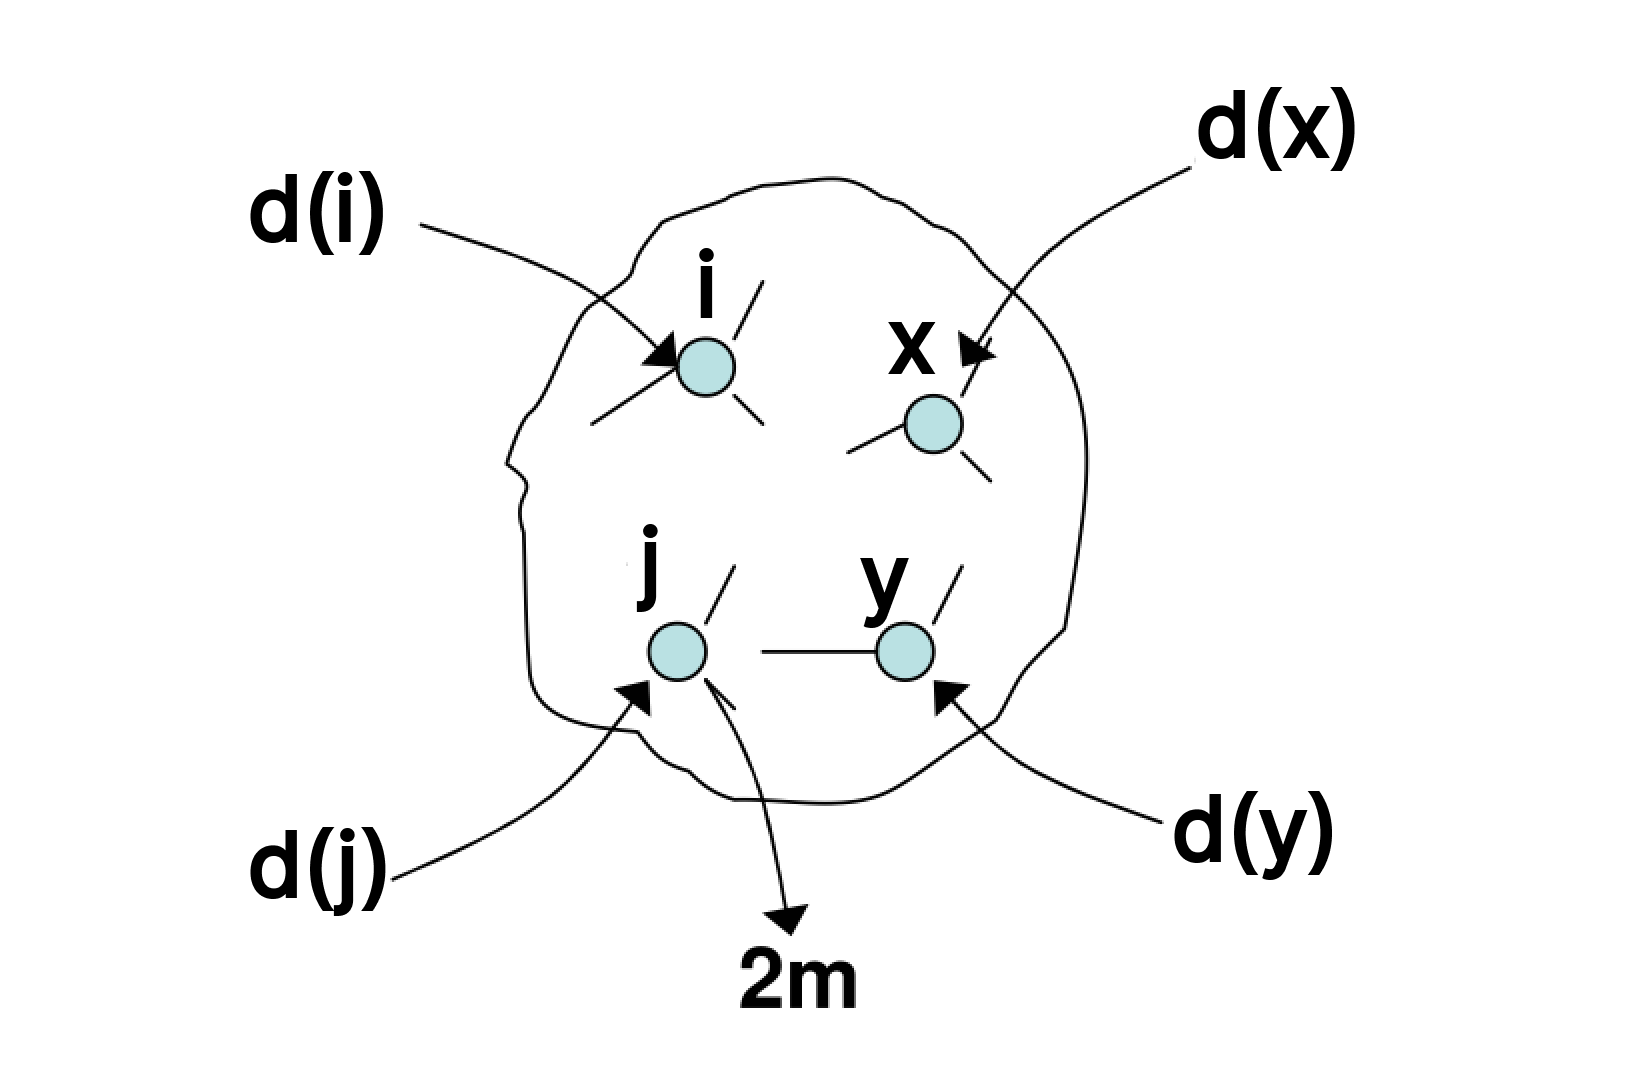
\includegraphics[width=0.3\linewidth]{figures/A.png}
    \caption{Сценарий A}
\end{figure}
\end{theorem}

Теорема взята из \cite{1}.

\begin{proof}

Для доказательства данной теоремы введем законы Кирхгофа и Ома:

\begin{itemize}
    \item Суммарный ток в вершине и из нее равен нулю (K1) \cite{4}
    \item Сумма разностей потенциалов в любом цикле равна нулю (K2) \cite{4}
    \item Ток, протекающий по любому ребру, равен \(\text{разности потенциалов} \text{ деленная на } \text{сопротивление}\) (Закон Ома) \cite{5}
\end{itemize}


Теперь рассмотрим любую вершину \(i \in V\). Используя законы Кирхгофа и Ома, мы имеем:

$$d(i) = \sum_{(i, x) \in E} \text{текущая } i \to x  \text{(K1)} $$
$$= \sum_{(i, x) \in E} \phi_{ix}   \text{(Закон Ома)} $$
$$= \sum_{(i, x) \in E} (\phi_{ij} - \phi_{xj}) \text{(K2)} $$
$$= d(i)\phi_{ij} - \sum_{(i, x) \in E} \phi_{xj} $$

Преобразование даст:

$$
\phi_{ij} = 
\begin{cases} 
0 &  i = j \\
1 + \frac{1}{d(i)} \sum\limits_{(i,x) \in E} \phi_{xj} &  i \neq j
\end{cases} 
\eqno(2)
$$


С другой стороны, рассмотрим случайное блуждание, начинающееся с \(i\). Рассматривая только первый шаг этой прогулки, мы видим, что время попадания \(H_{ij}\) удовлетворяет следующим условиям:

$$
H_{ij} = 
\begin{cases} 
0 &  i = j \\
1 + \frac{1}{d(i)} \sum\limits_{(i,x) \in E} H_{xj} &  i \neq j
\end{cases} 
\eqno(3)
$$

Но это точно такая же система линейных уравнений, как и (2), удовлетворяемая \(\phi_{ij}\). Поскольку мы знаем, что эта система имеет единственное решение (потенциалы однозначно определяются потоками тока), мы выводим, что:

$$H_{ij} =  \phi_{ij}  \forall i \in V  $$

\end{proof}

\section{Эффективное сопротивление}

Эффективное сопротивление (резистивное расстояние) \(\Omega_{vw}(\mathcal{L})\) между вершинами \(u\) и \(v\) в графе с равным сопротивлением \(r\) на всех рёбрах определяется как сумма взвешенных квадратов разностей между компонентами собственных векторов графа для всех пар узлов \(v\) и \(w\). В частности, для каждого узла \(v\) и \(w\) вычисляется разность компонент собственных векторов \(\psi_{jv}\) и \(\psi_{jw}\), которые соответствуют ненулевым собственным значениям \(\lambda_j(\mathcal{L})\) лапласиана. Затем, каждая разность возводится в квадрат, делится на соответствующее собственное значение, и все такие дроби суммируются для всех j от 2 до n. :

$$ \Omega_{vw}(\mathcal{L}) = \sum_{j=2}^{n} \frac{1}{\lambda_j(\mathcal{L})} (\psi_{jv} - \psi_{jw})^2 \eqno(4.1)$$


Данная запись присутствует в \cite{2} на стр. 11, но для  удобства, формула (4.1) будет видоизменена:


$$ R_{ij} = \sum_{k=1}^{n-1} \frac{(u_{ki} - u_{kj})^2}{\lambda_k} \eqno(4.2)$$


В формуле 4.2 \(\lambda_k\) – это собственные значения Лапласиана, где \(\lambda_0 = 0\), \(u_{ki}\) и \(u_{kj}\) - i-я и j-я компоненты k-го собственного вектора Лапласиана, а n – это вершины. Лапласиан, или матрица Лапласа определяется как матрица степеней \(D\) минус матрица смежности \(A\):
$$  \mathcal{L} = D - A  $$


\section{Время возвращения}
\begin{theorem}[Время возвращения]
Среднее время случайного перемещения из i в j и обратно определяется как cреднее время первого попадания в вершину \(j\) из вершины \(i\) плюс cреднее время первого попадания в вершину \(i\) из вершины \(j\) иле же как количество ребер \(m\) умноженное на эффективное сопротивление \(R_{ij}\) умноженное на два.

$$ C_{ij} = H_{ij} + H_{ji} = 2mR_{ij}\eqno(5)$$
\end{theorem}

Формула взята из \cite{3}, стр. 577.

\begin{proof}

Для доказательства используем сценарий B, который похож на сценарий A, за исключением того, что мы удаляем \(2m\) единицы тока с узла \(i\), а не с узла \(j\). Обозначая разность потенциалов в сценарии B через \(\phi^{'}\), мы имеем, согласно теореме 1:
$$\phi_{ji}^{'} = H_{ji} \eqno(6)$$

Теперь рассмотрим сценарий C, который похож на сценарий B, но с обратными токами. Обозначив разность потенциалов в этом сценарии через \(\phi''\), мы получаем:

$$\phi_{ij}^{''} = \phi_{ji}^{'} = H_{ji} \eqno(7)$$

\begin{figure}[h]
    \centering
    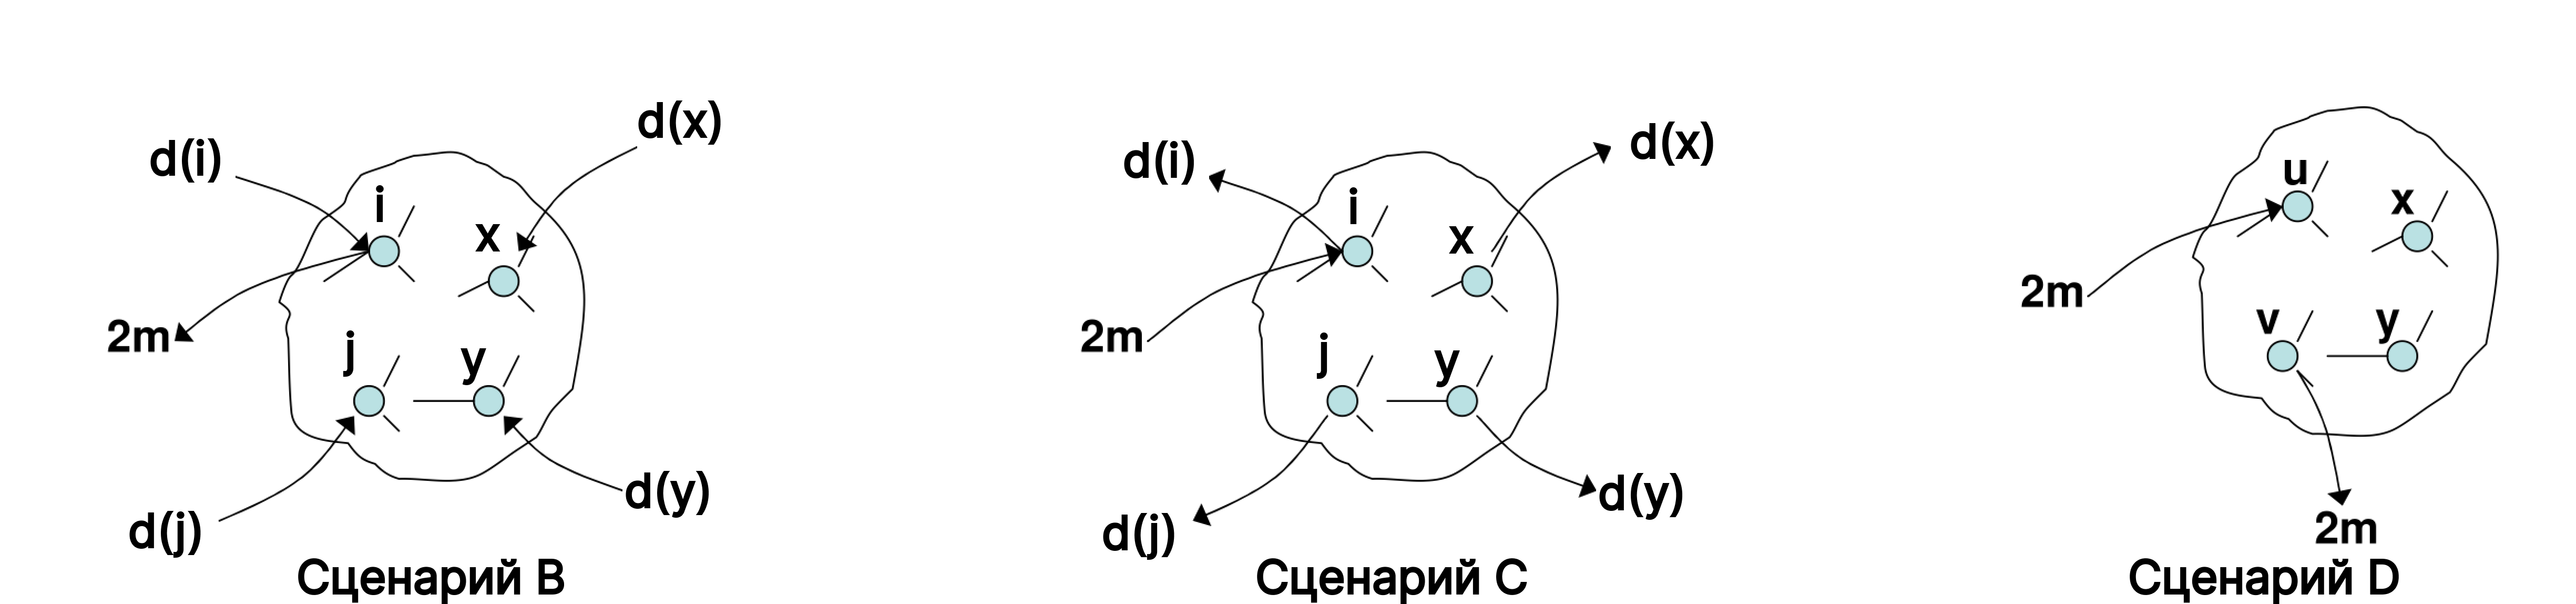
\includegraphics[width=1\linewidth]{figures/BCD.png}
    \caption{Сценарий B,C и D}
\end{figure}

Наконец, рассмотрим сценарий D, который представляет собой сумму сценариев A и C. В силу линейности и обозначения потенциальные различия в сценарии D через \(\phi^{'''}\), мы имеем:

$$\phi_{ij}^{'''} = \phi_{ij} + \phi_{ij}^{''}= H_{ij} = H_{ji} \eqno(8)$$

Так как \(\phi_{ij}^{''}\) – это разность потенциалов, необходимая для перемещения \(2m\) единиц тока из \(i\) в \(j\), поэтому по закону Ома она равна \(2mR_{ij}\).
\end{proof}


\chapter{Реализация программы}

\section{Переменные}
\subsection{Входные переменные}

\begin{itemize}
    \item \texttt{adj} - матрица смежности графа.
    \item \texttt{start} - индекс начального узла.
    \item \texttt{end_} - индекс конечного узла.
    \item \texttt{num_sim} - количество симуляций.
\end{itemize}

\subsection{Выходные переменные}

\begin{itemize}
    \item \texttt{fht} - вектор, содержащий время первого попадания в конечный узел для каждой симуляции.
    \item \texttt{ct} - вектор, содержащий время полного обхода графа для каждой симуляции.
    \item \texttt{cmt} - вектор, содержащий время перемещения от начального узла к конечному и обратно для каждой симуляции.
    \item \texttt{sfh} - отсортированный вектор времени первого попадания и их количества.
    \item \texttt{sct} - отсортированный вектор времени полного обхода графа и их количества.
    \item \texttt{scmt} - отсортированный вектор времени перемещения и их количества.
    \item \texttt{mfht} - среднее время первого попадания в конечный узел.
    \item \texttt{mct} - среднее время полного обхода графа.
    \item \texttt{mcmt} - среднее время перемещения от начального узла к конечному и обратно.
    \item \texttt{eff_res} - эффективное сопротивление графа, рассчитанное как среднее время перемещения, деленное на удвоенное количество ребер.
\end{itemize}

\subsection{Промежуточные переменные}

\begin{itemize}
    \item \texttt{n} - количество узлов в графе.
    \item \texttt{m} - количество ребер в графе, рассчитанное как половина суммы всех элементов матрицы смежности.
    \item \texttt{curr} - текущий узел в процессе блуждания.
    \item \texttt{visited} - булевый вектор, указывающий, были ли посещены узлы.
    \item \texttt{steps} - количество шагов, сделанных в текущей симуляции.
    \item \texttt{first_hit} - булева переменная, указывающая, было ли достигнуто первое попадание в конечный узел.
    \item \texttt{visit_count} - количество посещенных узлов.
    \item \texttt{neighbors} - вектор соседних узлов для текущего узла.
    \item \texttt{next} - следующий узел для перехода.
    \item \texttt{cms} - количество шагов для перемещения от начального узла к конечному и обратно в текущей симуляции.
    \item \texttt{file_path} - путь к файлу с матрицей смежности.
    \item \texttt{elapsed_time} - время, затраченное на выполнение симуляций.
\end{itemize}

\section{Скрипт random_walk.m}
В данной работе была разработана программа на языке Octave, которая имитирует случайные блуждания по графу, заданному матрицей смежности. Программа рассчитывает статистические данные. Об этих данных ниже рассказано более подробно. 


@d random_walk @{
function [fht, ct, sfh, sct, mfht, mct, eff_res, ...
mcmt, scmt] = random_walk(adj, start, end_, num_sim)
@< initialization of variables @>
@< simulation loop @>
@< calculation @>
@< sort function @>
@}
@o random_walk.oc @{@< random_walk  @>@}



В этом блоке инициализируются переменные для количества узлов и ребер в графе, векторов для хранения времени первого попадания, времени полного обхода, и времени перемещения.

@d initialization of variables @{
    n = size(adj, 1);
    m = sum(adj(:)) / 2;
    fht = zeros(num_sim, 1);
    ct = zeros(num_sim, 1);
    cmt = zeros(num_sim, 1);
@}

Этот блок выполняет цикл по числу симуляций для выполнения случайных блужданий.

@d simulation loop @{
@< initialising the current state @>
@< graph wandering cycle @>
@< hit check @>
@< update visited nodes @>
@< record round-trip time @>
@< calculation of travel time @>
@}

Этот блок начинает наш основной цикл, инициализируюя текущий узел как начальный узел , а также массивы для отслеживания посещенных узлов и количества шагов. Также инициализируются переменные для отслеживания первого попадания в конечный узел и количества посещенных узлов.

@d initialising the current state @{
    for sim = 1:num_sim
        curr = start;
        visited = false(n, 1);
        visited(start) = true;
        steps = 0;
        first_hit = false;
        visit_count = 1;
@}

Этот цикл продолжается до тех пор, пока не будут посещены все узлы графа. Внутри цикла определяется следующий узел для перехода случайным образом из соседей текущего узла.

@d graph wandering cycle @{
        while visit_count < n
            neighbors = find(adj(curr, :));
            next = neighbors(randi(length(neighbors)));
            steps = steps + 1;
            curr = next;
@}

Если это первое попадание в конечный узел, сохраняется количество шагов до первого попадания.

@d hit check @{
            if ~first_hit && curr == end_
                fht(sim) = steps;
                first_hit = true;
            end
@}

Если узел еще не был посещен, он помечается как посещенный, и увеличивается счетчик посещений.

@d update visited nodes @{
            if ~visited(curr)
                visited(curr) = true;
                visit_count = visit_count + 1;
            end
        end
@}

После завершения обхода всех узлов записывается количество шагов.

@d record round-trip time @{
        ct(sim) = steps;
@}

Затем рассчитывается время перемещения от начального узла к конечному и обратно. Это выполняется двумя циклами: один до конечного узла, и один обратно к начальному узлу.

@d calculation of travel time @{
        cms = 0;
        curr = start;
        while curr ~= end_
            neighbors = find(adj(curr, :));
            next = neighbors(randi(length(neighbors)));
            cms = cms + 1;
            curr = next;
        end
        while curr ~= start
            neighbors = find(adj(curr, :));
            next = neighbors(randi(length(neighbors)));
            cms = cms + 1;
            curr = next;
        end
        cmt(sim) = cms;
    end
@}

Здесь сортируются и подсчитываются вхождений для времени первого попадания, времени обхода и времени перемещения, используя вспомогательную функцию сортировки. Далее рассчитывается среднеее время первого попадания, среднее время обхода, среднее время перемещения и эффективное сопротивление.

@d calculation @{
    sfh = sort_and_count(fht);
    sct = sort_and_count(ct);
    scmt = sort_and_count(cmt);
    mfht = mean(fht);
    mct = mean(ct);
    mcmt = mean(cmt);

    eff_res = mcmt / (2 * m);
end
@}

Определение вспомогательной функции, которая сортирует данные и подсчитывает вхождения. Возвращает матрицу с отсортированными данными и их количеством.

@d sort function @{
function sc = sort_and_count(data)
    [sorted_data, ~, idx] = unique(data);
    counts = accumarray(idx, 1);
    sc = [sorted_data, counts];
end
@}

\section{Скрипт run_random_walk.m}
Для запуска функции random_walk и получения результатов был разработан скрипт run_random_walk. Этот скрипт задаёт параметры графа, запускает функцию random_walk и выводит результаты на экран.

@d run_random_walk @{
@< parameters set-up @>
@< running simulation@>
@< main results output @>
@< repeatable output hitting @>
@< repeatable output commute @>
@< repeatable output cover @>
@}
@o run_random_walk.oc @{@< run_random_walk  @>@}

Указание пути к файлу с матрицей смежности, начального узла, конечного узла и числа симуляций. Затем чтение матрицы смежности из указанного файла с помощью функции \texttt{dlmread} и сохранение в переменную матрицы смежности.

@d parameters set-up @{
file_path = 'adjacency_matrix.txt';
start = 1;
end_ = 442;
num_sim = 1000;

adj = dlmread(file_path);
@}

Выполнение функции случайного блуждания с заданными параметрами и измерение затраченного времени с помощью \texttt{tic} и \texttt{toc}. Результаты сохраняются в соответствующих переменных, а время выполнения - в переменной \texttt{elapsed_time}.

@d running simulation @{
tic;
[fht, ct, sfh, sct, mfht, mct, eff_res, mcmt, scmt] = random_walk(adj, start, end_, num_sim);
elapsed_time = toc;
@}


Этот блок кода выводит основные результаты вычислений, такие как: среднее время первого попадания, среднее время прохода, среднее время обхода всего графа, эффективное сопротивление, время выполнения программы

@d main results output  @{
fprintf('Среднее время первого попадания в вершину %d из вершины %d: %f шага.\n', end_, start, mfht);
fprintf('Среднее время прохода из вершины %d в вершину %d и обратно: %f шага.\n', start, end_, mcmt);
fprintf('Среднее время обхода всего графа: %f шага.\n', mct);
fprintf('Эффективное сопротивление: %f.\n', eff_res);
fprintf('Время выполнения программы: %f секунд.\n', elapsed_time);
@}


Следующий блок кода выводит детализированную информацию о повторениях времени для среднее время первого попадания.

@d repeatable output hitting @{
fprintf('Повторения времени первого попадания в вершину (в формате [время-количество]):\n');
    for i = 1:size(sfh, 1)
       fprintf('[%d-%d]', sfh(i, 1), sfh(i, 2));
       if i ~= size(sfh, 1)
           fprintf(', ');
       else
           fprintf('.\n');
       end
end
@}

Этот блок кода выводит детализированную информацию о повторениях времени для среднее время прохода.
@d repeatable output commute @{
fprintf('Повторения времени прохода из вершины %d в вершину %d и обратно (в формате [время-количество]):\n', start, end_);
    for i = 1:size(sfh, 1)
       fprintf('[%d-%d]', scmt(i, 1), scmt(i, 2));
       if i ~= size(sfh, 1)
           fprintf(', ');
       else
           fprintf('.\n');
       end
end
@}

А здесь выводится детализированную информацию о повторениях времени для среднее время обхода всего графа.
@d repeatable output cover @{
fprintf('Повторения времени обхода всего графа (в формате [время-количество]):\n');
    for i = 1:size(sfh, 1)
       fprintf('[%d-%d]', sct(i, 1), sct(i, 2));
       if i ~= size(sfh, 1)
           fprintf(', ');
       else
           fprintf('.\n');
       end
end
@}

\chapter{Результаты и их анализ}
\section{Проведение тестов}

В качестве примеров мы рассмотрим два графа. Первый граф будет тестовым для понимания методологии решения, а вторым графом является Московское метро.

\subsection{Практический пример 1}
\[
\text{adj_matrix} = \begin{pmatrix}
0 & 1 & 1 & 0 \\ 
1 & 0 & 1 & 1 \\ 
1 & 1 & 0 & 1 \\
0 & 1 & 1 & 0 
\end{pmatrix}
\]

Начальная вершина была выбрана как вершина 1, а конечная вершина как вершина 4. Количество симуляций было установлено на 1000. Результаты симуляций показали следующее:

\begin{itemize}
    \item Среднее время первого попадания в вершину 4 из вершины 1: 5.047200 шага.
    \item Среднее время прохода из вершины 1 в вершину 4 и обратно: 10.004400 шага.
    \item Среднее время обхода всего графа: 5.934400 шага.
    \item Эффективное сопротивление: 1.000440.
    \item Время выполнения программы: 7.940940 секунд.
    \item Повторения времени первого попадания в вершину 4 (в формате [время-количество]):
[2-3277], [3-1110], [4-1476], [5-881], [6-770], [7-578], [8-460], [9-346], [10-252], [11-198], [12-157], [13-116], [14-79], [15-69], [16-54], [17-33], [18-30], [19-27], [20-11], [21-8], [22-15], [23-7], [24-11], [25-11], [26-7], [27-4], [28-4], [29-2], [30-1], [31-1], [32-3], [36-1], [39-1].
    \item Повторения времени прохода из вершины 1 в вершину 4 и обратно (в формате [время-количество]):
[4-1141], [5-754], [6-1116], [7-857], [8-930], [9-813], [10-701], [11-579], [12-551], [13-458], [14-388], [15-340], [16-241], [17-193], [18-172], [19-149], [20-126], [21-102], [22-66], [23-72], [24-46], [25-50], [26-34], [27-24], [28-25], [29-14], [30-15], [31-8], [32-6], [33-8], [34-6], [35-3], [36-2], [38-1], [39-3], [40-2], [41-1], [43-1], [47-1], [54-1].
    \item Повторения времени обхода всего графа (в формате [время-количество]):
[3-2768], [4-1493], [5-1645], [6-959], [7-896], [8-538], [9-479], [10-288], [11-238], [12-175], [13-126], [14-86], [15-77], [16-54], [17-33], [18-30], [19-28], [20-11], [21-8], [22-15], [23-7], [24-11], [25-11], [26-7], [27-4], [28-4], [29-2], [30-1], [31-1], [32-3], [36-1], [39-1].
\end{itemize}
Стоит заметить, что при стократном увеличении симуляций, результаты изменятся лишь на немного, что можно посчитать как погрешность

\subsection{Практический пример 2}
В качестве второго примера будет взята матрица Московского метро, так как она позволит нам понять распределение случайных блужданий в реальной транспортной сети. Начальная вершина была выбрана как вершина 1, а конечная вершина как вершина 442. Количество симуляций было установлено на 100000. Результаты симуляций показали следующее:
\begin{itemize}
    \item Среднее время первого попадания в вершину 442 из вершины 1: 17159.75 шага.
    \item Среднее время прохода из вершины 1 в вершину 442 и обратно: 20142.68 шагаю
    \item Среднее время обхода всего графа: 40777.67 шага.
    \item Эффективное сопротивление: 15.99.
    \item Время выполнения программы: 3194.03 секунд.
    \item Повторения времени первого попадания в вершину 442 (в формате [время-количество]):
[181-1], [207-1], [223-1], [228-1], [247-1], [273-1], [283-1], [294-1], [295-1], [308-1], [310-1], [320-1], [326-1], [332-1], [347-1], [377-2], [380-1], [390-1], [394-1], [399-1], [403-1], [404-1], ..., [83303-1], [84775-1], [86292-1], [87511-1], [87871-1], [90300-1], [90512-1], [90706-1], [91685-1], [92204-1], [94005-1], [94046-1], [96670-1], [99268-1], [100331-1], [100423-1], [106359-1], [111794-1], [116396-1], [120840-1], [126162-1].
    \item Повторения времени прохода из вершины 1 в вершину 442 и обратно (в формате [время-количество]):
[664-1], [731-1], [896-1], [906-1], [951-1], [953-1], [1001-1], [1006-1], [1016-1], [1018-1], [1071-1], [1247-1], [1288-1], [1324-1], [1341-1], [1348-1], [1350-1], [1363-1], [1402-1], [1422-1], [1502-1], [1532-1], [1539-1], [1575-1], [1587-1], [1629-1], [1635-1], [1662-1], [1665-1], [1671-1], [1709-1], [1740-1], [1764-1], ..., [85889-1], [85916-1], [86833-1], [87254-1], [88314-1], [88847-1], [89007-1], [89170-1], [89626-1], [90126-1], [90970-1], [92160-1], [94804-1], [96182-1], [96784-1], [96859-1], [103180-1], [108376-1], [109164-1], [112139-1], [114772-1], [125381-1], [132213-1].
    \item Повторения времени обхода всего графа (в формате [время-количество]):
    [9647-1], [10655-1], [11128-1], [11480-1], [12063-1], [12111-1], [12701-1], [12790-1], [13708-1], [13803-1], [13859-1], [13917-1], [14018-1], [14119-1], [14238-1], [14321-1], [14353-1], [14437-1], [14468-1], [14512-1], [14611-1], [14617-1], [14844-1], [14956-1], [15062-1], [15243-1], [15263-1], [15273-1], [15327-2], [15402-1], [15504-1], [15646-1], [15666-1], [15695-1], [15697-1], [15726-1], [15746-1], ..., [102068-1], [102185-1], [102236-1], [102585-1], [103752-1], [104117-1], [104797-1], [105988-1], [106188-1], [[122495-1], [123046-1], [126162-1], [132426-1], [133163-1], [135711-1], [137445-1], [142049-1], [154437-1].
\end{itemize}

\section{Теоретические расчеты}
\subsection{Теоретический пример 1}
Теперь с помощью теории рассчитаем количество шагов до попадания в вершину 4 из вершины 1. Составим матрицу степеней из матрицы смежности, используемой выше:
\[
\text{D} = \begin{pmatrix}
2 & 0 & 0 & 0 \\ 
0 & 3 & 0 & 0 \\ 
0 & 0 & 3 & 0 \\
0 & 0 & 0 & 2 
\end{pmatrix}
\]

Из этих двух матриц составим матрицу Лапласа (Лапласиан), используя данную формулу: {L = D - adj_matrix}
\[
\begin{pmatrix}
2 & 0 & 0 & 0 \\ 
0 & 3 & 0 & 0 \\ 
0 & 0 & 3 & 0 \\
0 & 0 & 0 & 2 
\end{pmatrix}
-
\begin{pmatrix}
0 & 1 & 1 & 0 \\ 
1 & 0 & 1 & 1 \\ 
1 & 1 & 0 & 1 \\
0 & 1 & 1 & 0 
\end{pmatrix}
=
 \begin{pmatrix} 
2 & -1 & -1 & 0 \\ 
-1 & 3 & -1 & -1 \\ 
-1 & -1 & 3 & -1 \\
0 & -1 & -1 & 2 
\end{pmatrix} = \text{L}
\]

Далее мы получаем собственные значения и собственные вектора матрицы Лапласа, чтобы их получить я воспользуюсь Octave:

@d laplacian @{
laplacian_matrix = [2 -1 -1 0;                
                   -1 3 -1 -1;
                   -1 -1 3 -1;
                    0 -1 -1 2];


[eigenvectors, eigenvalues_matrix] = eig(laplacian_matrix);

eigenvalues = diag(eigenvalues_matrix);

disp('Собственные значения:');
disp(eigenvalues);

disp('Собственные вектора:');
disp(eigenvectors);
@}
@o laplacian.oc @{@< laplacian @>@}


Где eigenvalues – это \(\lambda_k\), а eigenvectors –  это  \(u_{i}\)

$$\lambda_1 = 0, \quad \lambda_2 = 2, \quad \lambda_3 = 4, \quad \lambda_4 = 4$$

\[
\text{U} =  \begin{pmatrix} 
-0.50 & -0.71 & 0.49 & 0.09 \\
-0.50 & 0.00 & -0.62 & 0.60 \\
-0.50 & 0.00 & -0.36 & -0.79 \\
-0.50 & 0.71 & 0.49 & 0.09 \\
\end{pmatrix} 
\]



У собственных значений убираем нулевое значения и берем нулевую и третью строки из матрицы \(U\) для расчета \(R_{14}\). Получаем следующее:
$$ \lambda_2 = 2, \quad \lambda_3 = 4, \quad \lambda_4 = 4 $$
$$ u_0  = (-0.50, -0.71, 0.49, 0.09)$$
$$ u_3  = (-0.50, 0.71, 0.49, 0.09)$$

Теперь нам нужны значения \(n\) и \(m\). У нас \(n\) уже известна, она равна 4, поэтому осталось найти \(m\). Для этого находим сумму всех элементов матрицы смежности и делим их на 2.

$$ \sum_{i,j} A_{ij} = 0 + 1 + 1 + 0 + 1 + 0 + 1 + 1 + 1 + 1 + 0 + 1 + 0 + 1 + 1 + 0 = 10$$

$$ E = \frac{10}{2} = 5$$

В итоге получаем, что \(m\) = 5 и \(n\) = 4. Получив эти значения, мы можем посчитать эффективное сопротивление, воспользуемся формулой (4.2):
$$ R_{14} = \sum_{k=1}^{n-1} \frac{(u_{k1} - u_{k4})^2}{\lambda_k} = \frac{(0.71 - (-0.71))^2}{2} + $$
$$ + \frac{(0.49 - 0.49)^2}{4} + \frac{(0.09 - 0.09)^2}{4} \approx 1.0082$$

Теперь нужно посчитать commute time, для этого воспользуемся формулой (5):

$$ C_{14} = 2mR_{14} = 2 * 5 * 1.0083 \approx 10.0082$$

Нам осталось посчитать только hitting time, но так как считая эту форуму в ручную мы получим не совсем точные значения, то предлагаю воспользоваться формулой (5):
$$ C_{14} = H_{14} + H_{41} $$
Для нашего маленького и симметричного графа, это равносильно что:
$$ C_{14} \approx 2H_{14} $$
Следовательно \(H_{14}\) равен:
$$ H_{14}  \approx \frac{C_{14} }{2} \approx \frac{10.0082}{2} \approx 5.0041$$ 

\subsection{Теоретические пример 2}
Пример 1 был приведен для демонстрации методологии. Поскольку нахождение вручную данных графа Московского метро практически невозможно, стоит воспользоваться программным методом. Для этого была написана программа, которая воспроизводит формулы, использованные выше, в виде алгоритмов.

@d theoretical_random_walk @{
@< parameters @>
@< calculation of eigenvalues and eigenvectors @>
@< parameters of the iterative process @>
@< neighbourhood lists @>
@< calculate the matrix H @>
@< calculation of results  @>
@< result output @>
@}
@o theoretical_random_walk.oc @{@< theoretical_random_walk @>@}


В этой части кода, мы загружаем матрицу смежности графа из файла. Затем определяем количество вершин и ребер.
@d parameters @{
file_path = 'moscow.txt';
adj_matrix = dlmread(file_path);

n = size(adj_matrix, 1);
m = sum(adj_matrix(:)) / 2;
@}


Здесь мы вычисляем по формулам собственные значения и собственные векторы. Далее извлекаем собственные значения в вектор. И отбрасываем первое нулевое собственное значение и соответствующий ему собственный вектор (они не нужны для дальнейших вычислений).

@d calculation of eigenvalues and eigenvectors @{
degree_matrix = sum(adj_matrix, 2);

laplacian_matrix = diag(degree_matrix) - adj_matrix;

[eigenvectors, eigenvalues_matrix] = eig(laplacian_matrix);
eigenvalues = diag(eigenvalues_matrix);

eigenvalues_nonzero = eigenvalues(2:end);
eigenvectors_nonzero = eigenvectors(:, 2:end);

@}

В этой части код инициализируем матрицу H нулями. Задаем максимальное количество итераций и допустимую ошибку.
@d parameters of the iterative process @{
H = zeros(n, n);

max_iter = 200000;
tol = 1e-16;
@}


Здесь начинаем подсчет времени выполнения. Затем создаем список соседей для каждой вершины. В каждой ячейке массива neighbors хранятся индексы соседей соответствующей вершины.

@d neighbourhood lists @{
tic;

neighbors = cell(n, 1);
for i = 1:n
    neighbors{i} = find(adj_matrix(i, :) == 1);
end
@}


В этом блоке в каждой итерации обновляем значения H для всех вершин, используя их соседей. Затем каждые 10000 итераций выводим текущую ошибку. Если ошибка становится меньше заданного порога (tol), процесс останавливается. И в конце записываем время выполнения итерационного процесса.
@d calculate the matrix H @{
for iteration = 1:max_iter
    H_prev = H;
    for u = 1:n
        if degree_matrix(u) > 0
            H(u, :) = 1 + (1 / degree_matrix(u)) * sum(H(neighbors{u}, :), 1);
        end
        H(u, u) = 0;  % Условие H_ii = 0
    end
    if mod(iteration, 10000) == 0
        disp(['Итерация: ', num2str(iteration), ' H - ', num2str(max(max(abs(H - H_prev))))]);
    end
    if max(max(abs(H - H_prev))) < tol
        disp(['Сошлось после ', num2str(iteration), ' итераций']);
        break;
    end
end
elapsed_time = toc;
@}


Здесь мы рассчитаем среднее время прохождения, время возвращения и эффективное сопротивление между заданными вершинами на основе полученных данных.
@d calculation of results @{
i = 1;
j = 421;

H_ij = H(i, j);

R_ij = sum((eigenvectors_nonzero(i, :) - eigenvectors_nonzero(j, :)).^2 ./ eigenvalues_nonzero');

C_ij = 2 * m * R_ij;
@}

Выводим вычисленные результаты.
@d result output @{
disp(['Среднее время прохода из вершины ', num2str(i), ' в вершину ', num2str(j), ': ', num2str(H_ij)]);
disp(['Среднее время прохода из вершины ', num2str(i), ' в вершину ', num2str(j), ' и обратно: ', num2str(C_ij)]);
disp(['Эффективное сопротивление: ', num2str(R_ij)]);
disp(['Время выполнения программы: ', num2str(elapsed_time), ' секунд']);
@}

 
 Результаты данных вычислений:
 \begin{itemize}
    \item Сошлось после 293492 итераций
    \item Среднее время прохождения из вершин 1 в вершину 442: 17085.752085552034
    \item Среднее время прохождения из вершины 1 в вершину 442 и обратно: 
    \item Эффективное сопротивление: 16.03125175687944
    \item Время выполнения программы: 2841.8106 секунд
\end{itemize}



\backmatter %% Здесь заканчивается нумерованная часть документа и начинаются 

\Conclusion

Результаты вычислительных экспериментов и теоретических расчетов для графа демонстрируют высокую степень согласованности, что свидетельствует о правильности и эффективности применяемых моделей и алгоритмов. Тестирование проводилось на графе с четырьмя вершинами, на котором было установлено, что теоретические предсказания совпадают с практическими результатами. Кроме того, применение данных методов на графе Московского метро показало, что алгоритмы могут эффективно работать не только в теоретических условиях, но и с реальной транспортной сетью. Среднее время первого попадания, прохождения и обхода всего графа, а также эффективное сопротивление, полученные в результате симуляций, находятся в хорошем согласии с теоретическими расчетами. Эти два случая подтверждают, что предложенные модели и алгоритмы могут быть успешно применены для анализа и прогнозирования поведения более сложных и масштабных транспортных сетей.

Высокая степень совпадения теоретических и практических результатов свидетельствует о том, что даже при увеличении размера графа выбранные алгоритмы остаются корректными и эффективными. Эти результаты позволяют сделать вывод о возможности масштабирования используемых методов на более крупные графы, сохраняя их точность и надежность.


\bibliographystyle{gost780u}
\bibliography{book}

\end{document}